\subsubsection{Experiments for Eliciting Boredom Emotion}

To explore boredom at different intensity levels, three carefully designed tasks were conducted. These tasks are grounded in psychological literature that identifies monotony, repetition, and lack of engagement as key contributors to boredom.

\paragraph*{Low-Intensity Boredom – Repetitive Button Clicking Task}

In the first task, participants were instructed to click a button at exact intervals over a duration of two minutes. This task is intentionally repetitive and minimally demanding, with no variation or challenge to stimulate cognitive engagement.

Boredom frequently arises from repetitive, purposeless actions that fail to engage mental resources~\citep{bench2013function}. This low-intensity task aligns with such conditions, offering minimal novelty and no meaningful outcome, which is expected to produce a mild but noticeable feeling of boredom due to understimulation.

\paragraph*{Medium-Intensity Boredom – Watching a Dripping Water Video}

The second task involves watching a video of water dripping from a tap for two minutes (\url{https://youtu.be/lVrYV0odeFY}) \citep{atomic_filmmaker_boring_video}. The visual stimulus is static and unchanging, offering no narrative or engaging content, which has been shown to reliably induce medium levels of boredom in controlled settings.

The use of unchanging visual stimuli is a validated method for boredom induction~\citep{markey2014identifying}. The slow, repetitive nature of the dripping water presents a low-information environment that sustains passive attention without mental engagement. Compared to the motor activity of button clicking, this passive viewing requires continuous focus but offers no new stimulation, making it suitable for inducing a moderate level of boredom~\citep{bench2013function}.

\paragraph*{High-Intensity Boredom – Watching a Yawning Video}

For high-intensity boredom, participants watched a two-minute video of someone yawning repeatedly (\url{https://youtu.be/M3QYDtSbhrA}) \cite{buzzfeed_yawning_video}. Yawning is closely associated with boredom, low arousal, and disengagement. Watching someone yawn repeatedly is likely to trigger similar responses in viewers, including physiological reactions like contagious yawning and a reduction in alertness.

Research has linked the act of yawning with increased feelings of boredom, drowsiness, and mind-wandering~\citep{norscia2020auditory}. The lack of narrative or engaging visual stimuli in the video is expected to amplify this effect. Additionally, contagious yawning may create a feedback loop of low arousal, further reinforcing the emotional state of boredom and making this task suitable for inducing high levels of boredom in participants.

Screenshots of the videos used in the experiments are shown in Figure~\ref{fig:task-boredom}. 

\begin{figure*}[h]
    \centering
    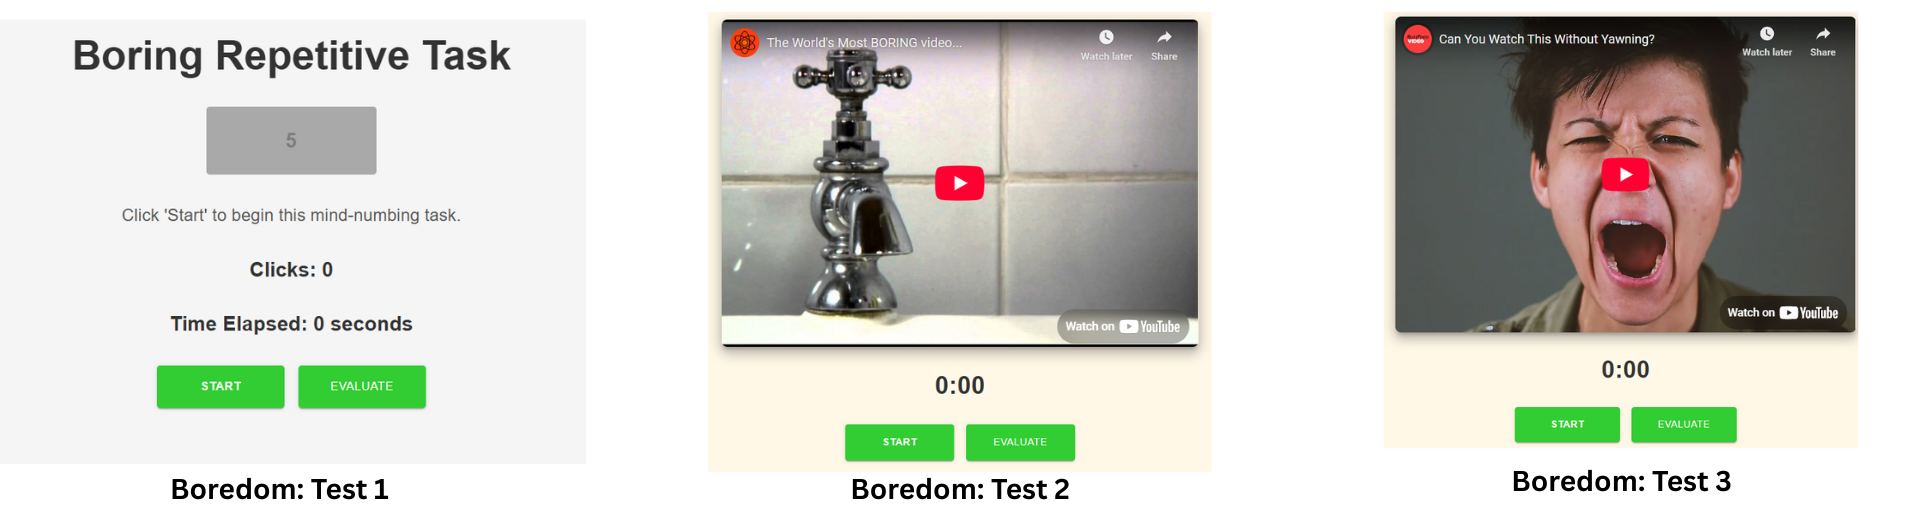
\includegraphics[width=1\textwidth]{img/chapter_03/boredom_tests.png}
    \captionof{figure}{Eliciting tasks for Boredem emotion}
    \label{fig:task-boredom}
\end{figure*}